%===============================================================================
% LaTeX sjabloon voor de bachelorproef toegepaste informatica aan HOGENT
% Meer info op https://github.com/HoGentTIN/latex-hogent-report
%===============================================================================

\documentclass[dutch,dit,thesis]{hogentreport}

% TODO:
% - If necessary, replace the option `dit`' with your own department!
%   Valid entries are dbo, dbt, dgz, dit, dlo, dog, dsa, soa
% - If you write your thesis in English (remark: only possible after getting
%   explicit approval!), remove the option "dutch," or replace with "english".

\usepackage{lipsum} % For blind text, can be removed after adding actual content

%% Pictures to include in the text can be put in the graphics/ folder
\graphicspath{{graphics/}}

%% For source code highlighting, requires pygments to be installed
%% Compile with the -shell-escape flag!
\usepackage[section]{minted}
%% If you compile with the make_thesis.{bat,sh} script, use the following
%% import instead:
%% \usepackage[section,outputdir=../output]{minted}
\usemintedstyle{solarized-light}
\definecolor{bg}{RGB}{253,246,227} %% Set the background color of the codeframe

%% Change this line to edit the line numbering style:
\renewcommand{\theFancyVerbLine}{\ttfamily\scriptsize\arabic{FancyVerbLine}}

%% Macro definition to load external java source files with \javacode{filename}:
\newmintedfile[javacode]{java}{
    bgcolor=bg,
    fontfamily=tt,
    linenos=true,
    numberblanklines=true,
    numbersep=5pt,
    gobble=0,
    framesep=2mm,
    funcnamehighlighting=true,
    tabsize=4,
    obeytabs=false,
    breaklines=true,
    mathescape=false
    samepage=false,
    showspaces=false,
    showtabs =false,
    texcl=false,
}

% Other packages not already included can be imported here

\usepackage{listings}
\usepackage{xcolor} % For syntax highlighting colors

%%---------- Document metadata -------------------------------------------------
% TODO: Replace this with your own information
\author{Emilio Tena Romero}
\supervisor{Dhr. S. Verschraege}
\cosupervisor{Dhr. G. Geens}
\title %[Optionele ondertitel]%
    {Inclusief Design: Optimalisatie van een kalenderapplicatie voor personen met Attention Deficit (Hyperactivity) Disorder.}
\academicyear{\advance\year by -1 \the\year--\advance\year by 1 \the\year}
\examperiod{1}
\degreesought{\IfLanguageName{dutch}{Professionele bachelor in de toegepaste informatica}{Bachelor of applied computer science}}
\partialthesis{false} %% To display 'in partial fulfilment'
%\institution{Internshipcompany BVBA.}

%% Add global exceptions to the hyphenation here
\hyphenation{back-slash}

%% The bibliography (style and settings are  found in hogentthesis.cls)
\addbibresource{bachproef.bib}            %% Bibliography file
\addbibresource{../voorstel/voorstel.bib} %% Bibliography research proposal
\defbibheading{bibempty}{}

%% Prevent empty pages for right-handed chapter starts in twoside mode
\renewcommand{\cleardoublepage}{\clearpage}

\renewcommand{\arraystretch}{1.2}

%% Content starts here.
\begin{document}

%---------- Front matter -------------------------------------------------------

\frontmatter

\hypersetup{pageanchor=false} %% Disable page numbering references
%% Render a Dutch outer title page if the main language is English
\IfLanguageName{english}{%
    %% If necessary, information can be changed here
    \degreesought{Professionele Bachelor toegepaste informatica}%
    \begin{otherlanguage}{dutch}%
       \maketitle%
    \end{otherlanguage}%
}{}

%% Generates title page content
\maketitle
\hypersetup{pageanchor=true}

%%=============================================================================
%% Voorwoord
%%=============================================================================

\chapter*{\IfLanguageName{dutch}{Woord vooraf}{Preface}}%
\label{ch:voorwoord}

%% TODO:
%% Het voorwoord is het enige deel van de bachelorproef waar je vanuit je
%% eigen standpunt (``ik-vorm'') mag schrijven. Je kan hier bv. motiveren
%% waarom jij het onderwerp wil bespreken.
%% Vergeet ook niet te bedanken wie je geholpen/gesteund/... heeft

\lipsum[1-2]
%%=============================================================================
%% Samenvatting
%%=============================================================================

% TODO: De "abstract" of samenvatting is een kernachtige (~ 1 blz. voor een
% thesis) synthese van het document.
%
% Een goede abstract biedt een kernachtig antwoord op volgende vragen:
%
% 1. Waarover gaat de bachelorproef?
% 2. Waarom heb je er over geschreven?
% 3. Hoe heb je het onderzoek uitgevoerd?
% 4. Wat waren de resultaten? Wat blijkt uit je onderzoek?
% 5. Wat betekenen je resultaten? Wat is de relevantie voor het werkveld?
%
% Daarom bestaat een abstract uit volgende componenten:
%
% - inleiding + kaderen thema
% - probleemstelling
% - (centrale) onderzoeksvraag
% - onderzoeksdoelstelling
% - methodologie
% - resultaten (beperk tot de belangrijkste, relevant voor de onderzoeksvraag)
% - conclusies, aanbevelingen, beperkingen
%
% LET OP! Een samenvatting is GEEN voorwoord!

%%---------- Nederlandse samenvatting -----------------------------------------
%
% TODO: Als je je bachelorproef in het Engels schrijft, moet je eerst een
% Nederlandse samenvatting invoegen. Haal daarvoor onderstaande code uit
% commentaar.
% Wie zijn bachelorproef in het Nederlands schrijft, kan dit negeren, de inhoud
% wordt niet in het document ingevoegd.

\IfLanguageName{english}{%
\selectlanguage{dutch}
\chapter*{Samenvatting}
\lipsum[1-4]
\selectlanguage{english}
}{}

%%---------- Samenvatting -----------------------------------------------------
% De samenvatting in de hoofdtaal van het document

\chapter*{\IfLanguageName{dutch}{Samenvatting}{Abstract}}

\lipsum[1-4]


%---------- Inhoud, lijst figuren, ... -----------------------------------------

\tableofcontents

% In a list of figures, the complete caption will be included. To prevent this,
% ALWAYS add a short description in the caption!
%
%  \caption[short description]{elaborate description}
%
% If you do, only the short description will be used in the list of figures

\listoffigures

% If you included tables and/or source code listings, uncomment the appropriate
% lines.
%\listoftables
%\listoflistings

% Als je een lijst van afkortingen of termen wil toevoegen, dan hoort die
% hier thuis. Gebruik bijvoorbeeld de ``glossaries'' package.
% https://www.overleaf.com/learn/latex/Glossaries

%---------- Kern ---------------------------------------------------------------

\mainmatter{}

% De eerste hoofdstukken van een bachelorproef zijn meestal een inleiding op
% het onderwerp, literatuurstudie en verantwoording methodologie.
% Aarzel niet om een meer beschrijvende titel aan deze hoofdstukken te geven of
% om bijvoorbeeld de inleiding en/of stand van zaken over meerdere hoofdstukken
% te verspreiden!

%%=============================================================================
%% Inleiding
%%=============================================================================

\chapter{\IfLanguageName{dutch}{Inleiding}{Introduction}}%
\label{ch:inleiding}

De inleiding moet de lezer net genoeg informatie verschaffen om het onderwerp te begrijpen en in te zien waarom de onderzoeksvraag de moeite waard is om te onderzoeken. In de inleiding ga je literatuurverwijzingen beperken, zodat de tekst vlot leesbaar blijft. Je kan de inleiding verder onderverdelen in secties als dit de tekst verduidelijkt. Zaken die aan bod kunnen komen in de inleiding~\autocite{Pollefliet2011}:

\begin{itemize}
  \item context, achtergrond
  \item afbakenen van het onderwerp
  \item verantwoording van het onderwerp, methodologie
  \item probleemstelling
  \item onderzoeksdoelstelling
  \item onderzoeksvraag
  \item \ldots
\end{itemize}

\section{\IfLanguageName{dutch}{Probleemstelling}{Problem Statement}}%
\label{sec:probleemstelling}

Uit je probleemstelling moet duidelijk zijn dat je onderzoek een meerwaarde heeft voor een concrete doelgroep. De doelgroep moet goed gedefinieerd en afgelijnd zijn. Doelgroepen als ``bedrijven,'' ``KMO's'', systeembeheerders, enz.~zijn nog te vaag. Als je een lijstje kan maken van de personen/organisaties die een meerwaarde zullen vinden in deze bachelorproef (dit is eigenlijk je steekproefkader), dan is dat een indicatie dat de doelgroep goed gedefinieerd is. Dit kan een enkel bedrijf zijn of zelfs één persoon (je co-promotor/opdrachtgever).

\section{\IfLanguageName{dutch}{Onderzoeksvraag}{Research question}}%
\label{sec:onderzoeksvraag}

Wees zo concreet mogelijk bij het formuleren van je onderzoeksvraag. Een onderzoeksvraag is trouwens iets waar nog niemand op dit moment een antwoord heeft (voor zover je kan nagaan). Het opzoeken van bestaande informatie (bv. ``welke tools bestaan er voor deze toepassing?'') is dus geen onderzoeksvraag. Je kan de onderzoeksvraag verder specifiëren in deelvragen. Bv.~als je onderzoek gaat over performantiemetingen, dan 

\section{\IfLanguageName{dutch}{Onderzoeksdoelstelling}{Research objective}}%
\label{sec:onderzoeksdoelstelling}

Wat is het beoogde resultaat van je bachelorproef? Wat zijn de criteria voor succes? Beschrijf die zo concreet mogelijk. Gaat het bv.\ om een proof-of-concept, een prototype, een verslag met aanbevelingen, een vergelijkende studie, enz.

\section{\IfLanguageName{dutch}{Opzet van deze bachelorproef}{Structure of this bachelor thesis}}%
\label{sec:opzet-bachelorproef}

% Het is gebruikelijk aan het einde van de inleiding een overzicht te
% geven van de opbouw van de rest van de tekst. Deze sectie bevat al een aanzet
% die je kan aanvullen/aanpassen in functie van je eigen tekst.

De rest van deze bachelorproef is als volgt opgebouwd:

In Hoofdstuk~\ref{ch:stand-van-zaken} wordt een overzicht gegeven van de stand van zaken binnen het onderzoeksdomein, op basis van een literatuurstudie.

In Hoofdstuk~\ref{ch:methodologie} wordt de methodologie toegelicht en worden de gebruikte onderzoekstechnieken besproken om een antwoord te kunnen formuleren op de onderzoeksvragen.

% TODO: Vul hier aan voor je eigen hoofstukken, één of twee zinnen per hoofdstuk

In Hoofdstuk~\ref{ch:conclusie}, tenslotte, wordt de conclusie gegeven en een antwoord geformuleerd op de onderzoeksvragen. Daarbij wordt ook een aanzet gegeven voor toekomstig onderzoek binnen dit domein.
\chapter{\IfLanguageName{dutch}{Stand van zaken}{State of the art}}%
\label{ch:stand-van-zaken}

% Tip: Begin elk hoofdstuk met een paragraaf inleiding die beschrijft hoe
% dit hoofdstuk past binnen het geheel van de bachelorproef. Geef in het
% bijzonder aan wat de link is met het vorige en volgende hoofdstuk.

% Pas na deze inleidende paragraaf komt de eerste sectiehoofding.

Dit hoofdstuk bevat je literatuurstudie. De inhoud gaat verder op de inleiding, maar zal het onderwerp van de bachelorproef *diepgaand* uitspitten. De bedoeling is dat de lezer na lezing van dit hoofdstuk helemaal op de hoogte is van de huidige stand van zaken (state-of-the-art) in het onderzoeksdomein. Iemand die niet vertrouwd is met het onderwerp, weet nu voldoende om de rest van het verhaal te kunnen volgen, zonder dat die er nog andere informatie moet over opzoeken \autocite{Pollefliet2011}.

Je verwijst bij elke bewering die je doet, vakterm die je introduceert, enz.\ naar je bronnen. In \LaTeX{} kan dat met het commando \texttt{$\backslash${textcite\{\}}} of \texttt{$\backslash${autocite\{\}}}. Als argument van het commando geef je de ``sleutel'' van een ``record'' in een bibliografische databank in het Bib\LaTeX{}-formaat (een tekstbestand). Als je expliciet naar de auteur verwijst in de zin (narratieve referentie), gebruik je \texttt{$\backslash${}textcite\{\}}. Soms is de auteursnaam niet expliciet een onderdeel van de zin, dan gebruik je \texttt{$\backslash${}autocite\{\}} (referentie tussen haakjes). Dit gebruik je bv.~bij een citaat, of om in het bijschrift van een overgenomen afbeelding, broncode, tabel, enz. te verwijzen naar de bron. In de volgende paragraaf een voorbeeld van elk.

\textcite{Knuth1998} schreef een van de standaardwerken over sorteer- en zoekalgoritmen. Experten zijn het erover eens dat cloud computing een interessante opportuniteit vormen, zowel voor gebruikers als voor dienstverleners op vlak van informatietechnologie~\autocite{Creeger2009}.

Let er ook op: het \texttt{cite}-commando voor de punt, dus binnen de zin. Je verwijst meteen naar een bron in de eerste zin die erop gebaseerd is, dus niet pas op het einde van een paragraaf.

\lipsum[7-20]

%%=============================================================================
%% Methodologie
%%=============================================================================

\chapter{\IfLanguageName{dutch}{Methodologie}{Methodology}}%
\label{ch:methodologie}

%% TODO: In dit hoofstuk geef je een korte toelichting over hoe je te werk bent
%% gegaan. Verdeel je onderzoek in grote fasen, en licht in elke fase toe wat
%% de doelstelling was, welke deliverables daar uit gekomen zijn, en welke
%% onderzoeksmethoden je daarbij toegepast hebt. Verantwoord waarom je
%% op deze manier te werk gegaan bent.
%% 
%% Voorbeelden van zulke fasen zijn: literatuurstudie, opstellen van een
%% requirements-analyse, opstellen long-list (bij vergelijkende studie),
%% selectie van geschikte tools (bij vergelijkende studie, "short-list"),
%% opzetten testopstelling/PoC, uitvoeren testen en verzamelen
%% van resultaten, analyse van resultaten, ...
%%
%% !!!!! LET OP !!!!!
%%
%% Het is uitdrukkelijk NIET de bedoeling dat je het grootste deel van de corpus
%% van je bachelorproef in dit hoofstuk verwerkt! Dit hoofdstuk is eerder een
%% kort overzicht van je plan van aanpak.
%%
%% Maak voor elke fase (behalve het literatuuronderzoek) een NIEUW HOOFDSTUK aan
%% en geef het een gepaste titel.

In deze sectie zal het volledige proces van het ontwikkelen van de kalender worden besproken. \newline

Om te beginnen zullen de eisen worden geprioriteerd met behulp van de MoSCoW-methode. Hierbij worden ze ingedeeld in vier categorieën: Must-have, Should-have, Could-have, en Won't-have. Daarna zal een applicatie ontwikkeld worden die grotendeels aan deze eisen voldoet, rekening houdend met de beperkingen in tijd en middelen. \newline

Voor het maken van de proof of concept zal een stappenplan worden opgebouwd voor het ontwikkelen van een eenvoudige kalenderapplicatie, inclusief de integratie van specifieke extra eisen. Ook een link naar de GitHub-repository van de uiteindelijke applicatie zal beschikbaar zijn. Zodat degenen die het onderzoek willen voortzetten of de applicatie verder willen ontwikkelen gemakkelijk een totale toegang hebben tot de ontwikkelde applicatie.

\section{MoSCoW-Methode}
Uit de lijst opgesteld in de literatuurstudie kan meteen worden afgeleid dat de belangrijkste functionaliteiten van de kalender alles is dat te maken heeft met het plannen. Deze zullen bij de must-have worden geplaatst omdat dit noodzakelijk is om een kalender te kunnen zijn. Bij de should-have zullen de zaken worden geplaatst die de Quality of Life (QoL) verhogen zoals de inclusieve oplossing die gevonden werden, namelijk de Brain Dump, overzicht van taken, etc. \newline

Bij de could-have van deze Proof of Concept zullen vooral zaken zitten die niet ontwikkeld gaan worden tijdens het onderzoek, maar er later zeker bij kunnen komen zoals een groepskalender die gesynchroniseerd is met die van andere personen of het importeren van externe kalenders.  De won't-have is nog niet echt besproken maar hier zullen zaken bij horen die absoluut vermeden moeten worden omdat ze voor te veel afleiding zorgen. \newline

Dan ziet de geprioriteerde lijst van eisen aan de hand van de MoSCoW-methode er als volgt uit:

\subsection{Must have}

    \begin{itemize}
        \item 	Weekoverzicht
        \item 	Maandoverzicht
        \item 	Planning raadplegen
        \item 	Taken toevoegen
        \item 	Afspraken en andere zaken kunnen inplannen
        \item 	Ingeplande taken, afspraken en andere zaken kunnen raadplegen
        \item 	Taken, afspraken en ander ingeplande zaken kunnen beheren (aanpassen, verwijderen, …)
    \end{itemize}


\subsection{Should have}

    \begin{itemize}
        \item	‘Andere zaken’, events, taken en afspraken kunnen opdelen in categorieën
        \item	Navigeren tussen weken, maanden, jaren (afhankelijk van view)
        \item	Overzicht van alle in te plannen taken/ events
        \item	Toevoegen van een ‘Brain Dump’ 
        \item	Prioritering van taken
        \item	Een badge verdienen bij het verrichten van taken
        \item	Mogelijkheid om grote/ lange taken op te delen in kleinere taken
        \item	Categorieën een kleur geven
        \item	Notificaties 
    \end{itemize}
    

\subsection{Could have}

    \begin{itemize}
        \item 	Groepskalender
        \item 	Jaaroverzicht
        \item 	Mogelijkheden om taken, afspraken en andere zaken te herhalen voor x aantal dagen/ weken/ maanden
        \item 	Externe kalenders importeren
        \item 	Light/Dark mode 
    \end{itemize}
    
    
\subsection{Won't have}

    \begin{itemize}
        \item	Advertenties
        \item	Pop-ups
        \item	Links naar externe sociale media
         
    \end{itemize}


Nu de vereisten duidelijk zijn gespecificeerd, is het tijd om over te gaan naar de ontwikkeling van de Proof of Concept. Het volgende hoofdstuk zal een selectie presenteren van de requirements die in de voorgaande sectie zijn geordend. \newline

De opbouw van de proof of concept zal stap voor stap worden overlopen, te beginnen met de voorbereiding van de gebruikersinterface (UI) en lay-out.  \newline
Vervolgens zullen we de ontwikkeling behandelen, waarbij we de benodigde vereisten voor de opbouw van een simpele applicatie implementeren en functionaliteiten toevoegen om aan de gestelde eisen te voldoen. \newline

Nadat de Proof of Concept is opgebouwd, zal deze online worden gezet en getest worden door de doelgroep aan de hand van een evaluatieformulier. \newline
Daarna zullen we alle verkregen resultaten analyseren en de nodige conclusies trekken met betrekking tot de ontworpen features.


\chapter{\IfLanguageName{dutch}{Proof Of Concept}{Proof Of Concept}}%
\label{ch:proofofconcept}

In dit stukje gaat er stap per stap beschreven worden hoe de testapplicatie zal worden opgebouwd. Deze zal een handleiding bevatten om de applicatie ook zelf te kunnen ontwikkelen, en er is ook een link naar de GitHub-Repository \footnote{GitHub Repo: \url{https://github.com/EmilioTR/kalenderapplicatie}.} van de volledig afgewerkte applicatie beschikbaar.


\section{Voorbereiden}

Voor dat we beginnen met de applicatie te ontwikkelen is het eerst belangrijk om vast te leggen welke requirements erin gaan zitten en hoe de kalender er gaat uitzien qua lay-out. \newline

Met behulp van de lijst met eisen verkregen door de MoSCoW-methode, is het nu eenvoudig te bepalen welke onderdelen in de applicatie worden opgenomen. We zullen alle 'must-haves' en 'should-haves' integreren, met uitzondering van 'notificaties' en 'prioritering van taken'. Deze twee functies worden uitgesloten omdat een notificatiesysteem voor deze proof of concept niet noodzakelijk is, en omdat de implementatie van taakprioritering meer tijd in beslag zou nemen dan nodig is om een testbare applicatie te ontwikkelen. Het is een functie die later nog altijd kan worden toegevoegd.\newline

Nu we weten welke functies we willen implementeren, kunnen we beginnen met het ontwerpen van de lay-out van de applicatie. Het ontwerp moet eenvoudig, overzichtelijk en gebruiksvriendelijk zijn. Om dit te bereiken, zullen we een beperkt aantal grote en duidelijke knoppen gebruiken. De hele functionaliteit moet intuïtief zijn, zodat gebruikers er gemakkelijk mee overweg kunnen en hun doelen kunnen bereiken met een minimaal aantal klikken. Dit kan worden bereikt door de belangrijkste functies op één scherm te plaatsen, zonder het te druk te maken. \newline

Om dit te bereiken en het overzichtelijk te houden, kunnen we hulpmiddelen gebruiken zoals een dialoogvenster voor het beheren van evenementen en een zijmenu ("drawer") voor extra functies zoals een "Brain Dump".  \newline

Door het gebruik van sobere kleuren blijft de app rustig en aangenaam om naar te kijken. De categorie kleuren daarentegen mogen sterk van contrast zijn om zo een duidelijk verschil te geven tussen het soort evenementen, wat ook helpt bij het overzicht en de duidelijkheid van alles dat is ingepland. \newline

Voor een eerste visuele weergave van het ontwerp worden er mock-up’s gemaakt (zie Figuur 4.1 en 4.2). De verkozen themakleur is pastelviolet, deze is zeer neutraal en zorgt voor een rustige omgeving.

\begin{figure}[h]
    \centering
    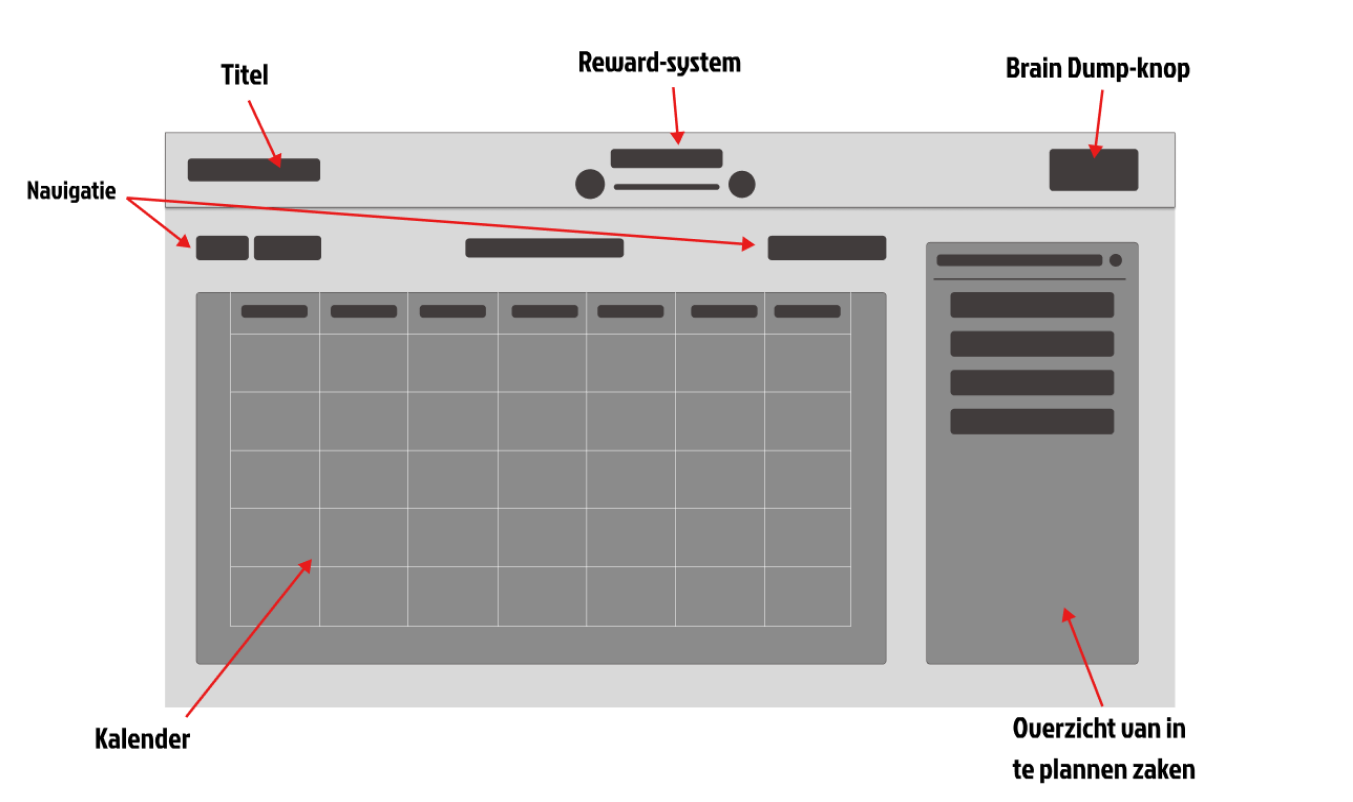
\includegraphics[width=\textwidth]{graphics/mockup_kalender.png}
    \caption{Mockup van de kalenderapplicatie.}
    \label{fig:mockup_app}
\end{figure}

\begin{figure}[h]
    \centering
    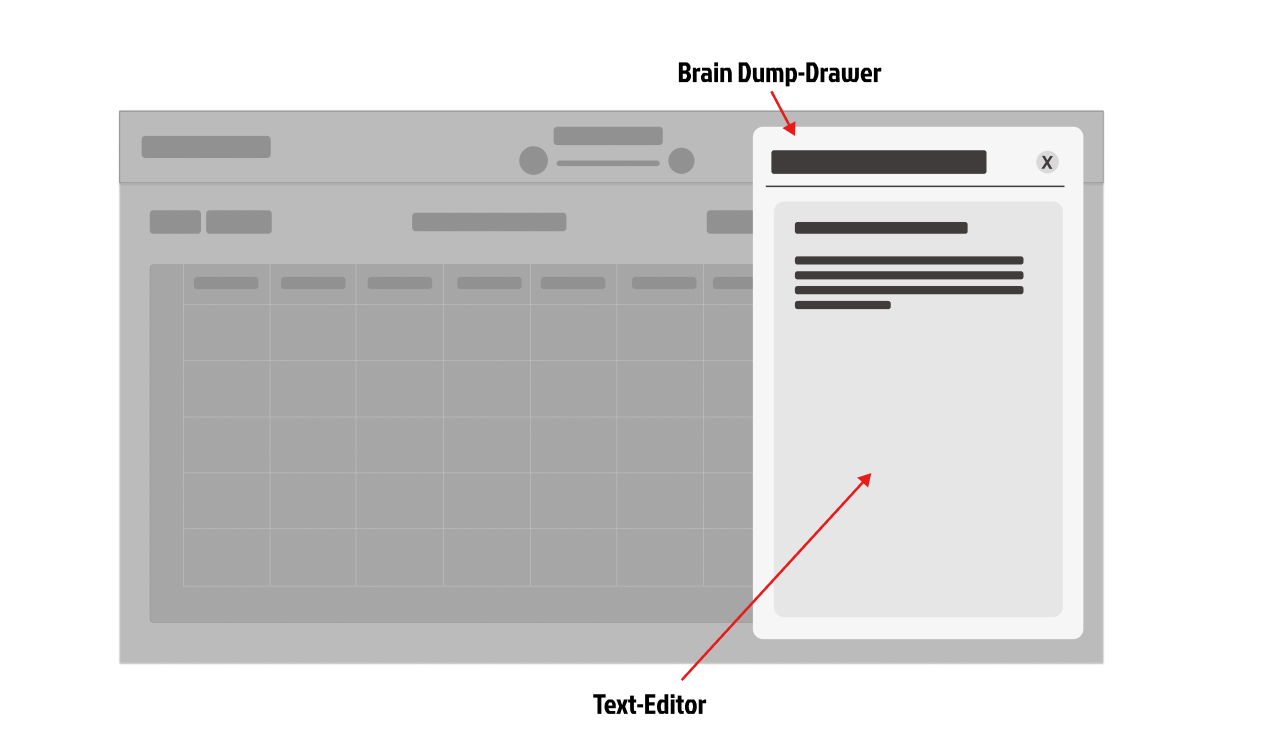
\includegraphics[width=\textwidth]{graphics/mockup_braindump.png} 
    \caption{Mockup van de Brain Dump functie.}
    \label{fig:mockup_braindump}
\end{figure}


\section{Opbouw van de applicatie}

De Proof of Concept zal worden ontwikkeld als een webapplicatie, wat de bruikbaarheid en implementatie ervan aanzienlijk vergemakkelijkt. De keuze voor het ontwikkelingsframework valt op 'Next.js', een veelgebruikt JavaScript-framework voor het bouwen van “single page applications”. En als IDE zal er gekozen worden voor Visual Studio Code. \newline

De beslissing om voor Next.js te kiezen komt voort uit verschillende overwegingen. Allereerst maakt Next.js het zeer eenvoudig om de applicatie online te hosten dankzij de ingebouwde server-side rendering. Bovendien vereenvoudigt het framework het beheer van de backend, wat van cruciaal belang kan zijn in latere ontwikkelingsfasen, vooral als er met een database moet worden geïntegreerd.  \newline

Hoewel deze proof of concept geen backend zal hebben en er geen permanente gegevensopslag naar een database zal plaatsvinden, zal alles operationeel zijn met testgegevens uit een JSON-bestand. Echter biedt het gebruik van Next.js de flexibiliteit om in de toekomst eenvoudig over te schakelen naar een meer geavanceerde backend-architectuur, mocht dat nodig zijn.

\subsection{Vereisten voor de ontwikkeling}

Om een applicatie te kunnen maken in Next.js \footnote{Next.js: \url{https://nextjs.org/}.} gaan we deze eerst moeten installeren. Dit kan heel gemakkelijk als volgt:

\begin{enumerate}
    \item	Open een nieuw terminalvenster in de folder waar de applicatie zal worden ontwikkeld.
    \item	Voer het volgende commando uit: `npx create-next-app@latest`.
    \item	Volg de prompts die verschijnen en selecteer voor alle opties de standaardinstellingen, behalve voor de "src/" directory, die moet wel worden toegevoegd.
\end{enumerate}

Na voltooiing van deze stappen zal een gestructureerde mappenhiërarchie worden aangemaakt in de opgegeven map, inclusief de noodzakelijke basisafhankelijkheden voor de werking van de applicatie.\newline

Om de ontwikkeling van de applicatie efficiënter te laten verlopen, maken we gebruik van bestaande React-libraries in plaats van alles vanaf nul op te bouwen. De volgende libraries worden gebruikt:

\begin{itemize}[label=$\rightarrow$]
    \item FullCalendar React \footnote{FullCalendar:      \url{https://www.npmjs.com/package/@fullcalendar/react}.}
    \item MUI Core \footnote{MUI Core: \url{https://mui.com/core/}.}
    \begin{itemize}[label=-]
        \item MUI Material 
        \item MUI Joy
        \item MUI Icons-Material
    \end{itemize}
    
    \item HeadlessUI React \footnote{HeadlessUI: \url{https://headlessui.com/}.}
    \item React Novel (lightweight version)  \footnote{Novel lightweight: \url{https://github.com/Ankur-Datta-4/novel-lightweight}.}
\end{itemize}

Deze libraries kunnen worden geïnstalleerd met behulp van het commando `npm install <naam-package>`. Een uitgebreide installatiehandleiding is te vinden op de respectieve webpagina's van de libraries.

\subsection{Implementatie}

Deze sectie presenteert een basisimplementatie van de kalender en de relevante functies voor dit onderzoek, namelijk de inclusieve features gevonden tijdens het onderzoek. Er zal geen uitgebreide code worden getoond; in plaats daarvan wordt een beknopt overzicht gegeven van het gebruik en de vereiste opties. Voor de volledige code wordt verwezen naar de publieke GitHub Repository \footnote{GitHub Repo: \url{https://github.com/EmilioTR/kalenderapplicatie}.}. \newline
De relevante functies die geïmplementeerd worden zijn de volgende: De Braindump, Overzicht van in te plannen zaken en een beloningssysteem (voor deze proof of concept een badge systeem dus)

\subsubsection{Kalender}

Voor de kalender wordt FullCalendar React gebruikt, een bibliotheek die een volledig operationele kalender biedt. Uit de vele beschikbare functionaliteiten zijn specifieke functies geselecteerd voor deze proof of concept. Deze worden in het codeblok hieronder getoond en toegelicht

\begin{lstlisting}[language=JavaScript, caption={Code Snippet - Kalender}, label={lst:codesnippet1}, frame=single, breaklines=true, backgroundcolor=\color{lightgray}]
    
    import FullCalendar from "@fullcalendar/react";
    import dayGridPlugin from '@fullcalendar/daygrid'
    import interactionPlugin, { Draggable, DropArg } from '@fullcalendar/interaction'
    import timeGridPlugin from '@fullcalendar/timegrid'
    import listPlugin from '@fullcalendar/list'
    import nlLocale from "@fullcalendar/core/locales/nl";
    
    ...
    
    <FullCalendar
    plugins={[
        dayGridPlugin,
        interactionPlugin,
        timeGridPlugin,
        listPlugin
        ]}
    headerToolbar={{
            left: 'prev,next today',
            center: 'title',
            right: 'timeGridWeek,dayGridMonth,listWeek'
    }}
    locale={nlLocale}
    events={allTodos as EventSourceInput}
    initialView='timeGridWeek'
    nowIndicator={true}
    editable={true}
    droppable={true}
    selectable={true}
    selectMirror={true}
    dateClick={handleDateClick}
    select={(data) => handleDateSelect(data)}
    drop={(data) => addTodo(data)}
    eventClick={(data) => handleShowModal(data)}
    eventResize={(info) => handleEventResize(info)}
    eventDrop={(info) => handleEventResize(info)}
    />
    
\end{lstlisting}
De nadruk ligt hierbij op de opties die het proces van het maken en aanpassen van evenementen in de kalender vergemakkelijken. Zoals de ‘eventResize’ bijvoorbeeld, deze zorgt ervoor dat telkens een event langer wordt gemaakt door het slepen, dit correct gebeurt. De implementatie van de ‘handleEventResize()’ methode zal hier niet uitgelegd worden, naar deze bevat de logica om het aangepaste event correct op te slaan. \newline

Bovenaan worden de vereiste plug-ins vermeld en wordt aangegeven hoe deze geïmporteerd moeten worden. De 'Header Toolbar' verwijst naar de interactieknoppen boven de kalender, die onder andere navigatieknoppen bevatten om tussen maanden/weken te kunnen schakelen, evenals knoppen om de weergave te wijzigen tussen week, maand en lijst. \newline

De opties die in deze code zijn gekozen omvatten respectievelijk een 'terug-knop', een 'volgende-knop', een titel die de geselecteerde maand/week aanduidt, en tot slot de drie knoppen om de weergave te veranderen.\newline

Het resultaat van de kalender met volledige implementatie en gepaste styling ziet er als volgt uit (figuur 4.3):

\begin{figure}[h]
    \centering
    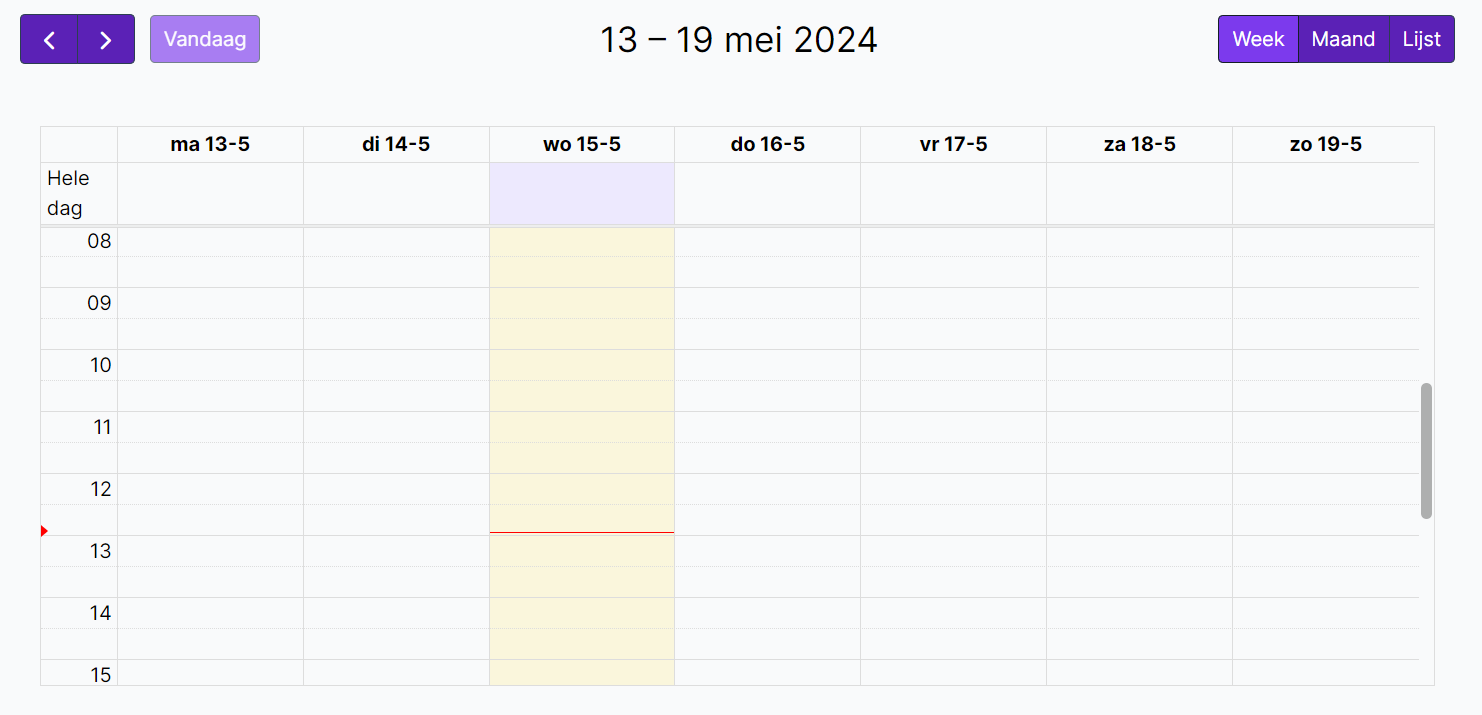
\includegraphics[width=\textwidth]{graphics/screenshot_kalender.png}
    \caption{Screenshot van de kalender.}
    \label{fig:screenshot_kalender}
\end{figure}


\subsubsection{Braindump}

Voor de Braindump zijn verschillende componenten gebruikt, waarbij gebruik is gemaakt van externe bibliotheken om deze correct te laten functioneren. Onder andere zijn een Drawer-, Dialog- en Sheet-component uit de MUI-bibliotheek geïmporteerd. Deze componenten worden ingezet om een venster aan de zijkant te laten verschijnen wanneer er op de desbetreffende ‘Braindump-knop’ wordt gedrukt. Op deze manier wordt de lay-out overzichtelijk gehouden en voorkomen we dat het te druk wordt.\newline

Voor de teksteditor die zich in dit uitklapbare venster bevindt, wordt gebruik gemaakt van de React Novel Lightweight-bibliotheek. Hiermee kan een ruimte gecreëerd worden die functionaliteiten biedt vergelijkbaar met Notion, waarbij het gevoel wordt gecreëerd alsof men op papier schrijft met de mogelijkheid tot het eenvoudig maken van lijsten, markeren, kleurcoderen, afbeeldingen invoegen, enzovoorts.\newline

Het implementeren van deze componenten ziet er als volgt uit: 

\begin{lstlisting}[language=JavaScript, caption={Code Snippet - Brain Dump Drawer}, label={lst:codesnippet2}, frame=single, breaklines=true, backgroundcolor=\color{lightgray}]
    
import Drawer from '@mui/joy/Drawer';
import ModalClose from '@mui/joy/ModalClose';
import DialogTitle from '@mui/joy/DialogTitle';
import DialogContent from '@mui/joy/DialogContent';
import Sheet from '@mui/joy/Sheet';
import Divider from '@mui/joy/Divider';
import BrainDumpEditor from '@/components//braindump/brainDumpEditor'


export default function BrainDumpDrawer({ openDrawer, setOpenDrawer }) {
    
    return (
    <Drawer
    open={openDrawer}
    onClose={() => setOpenDrawer(false)}
    anchor='right'
    size='lg'
    >
    
    <Sheet
    sx={{ /* Styling */ }}
    >
    <ModalClose />
    <DialogTitle>Brain Dump</DialogTitle>
    <Divider/>
    <DialogContent>
    <BrainDumpEditor />
    </DialogContent>
    </Sheet>
    </Drawer>
    )
    
}

\end{lstlisting}

\begin{lstlisting}[language=JavaScript, caption={Code Snippet - Text Editor}, label={lst:codesnippet3}, frame=single, breaklines=true, backgroundcolor=\color{lightgray}]
    
    import { Editor } from "novel-lightweight";
    import { useState } from "react";
    
    export default function BrainDumpEditor() {
        const [data, setData] = useState('');
        
        return (
        <Editor
        defaultValue={data}
        disableLocalStorage={false}
        onUpdate={(editor) => {
                setData(editor?.storage.markdown.getMarkdown());
        }}
        />
        );
    }
    
\end{lstlisting}

Het resultaat van de Braindump met volledige implementatie en gepaste styling ziet er als volgt uit (figuur 4.4):

\begin{figure}[h]
    \centering
    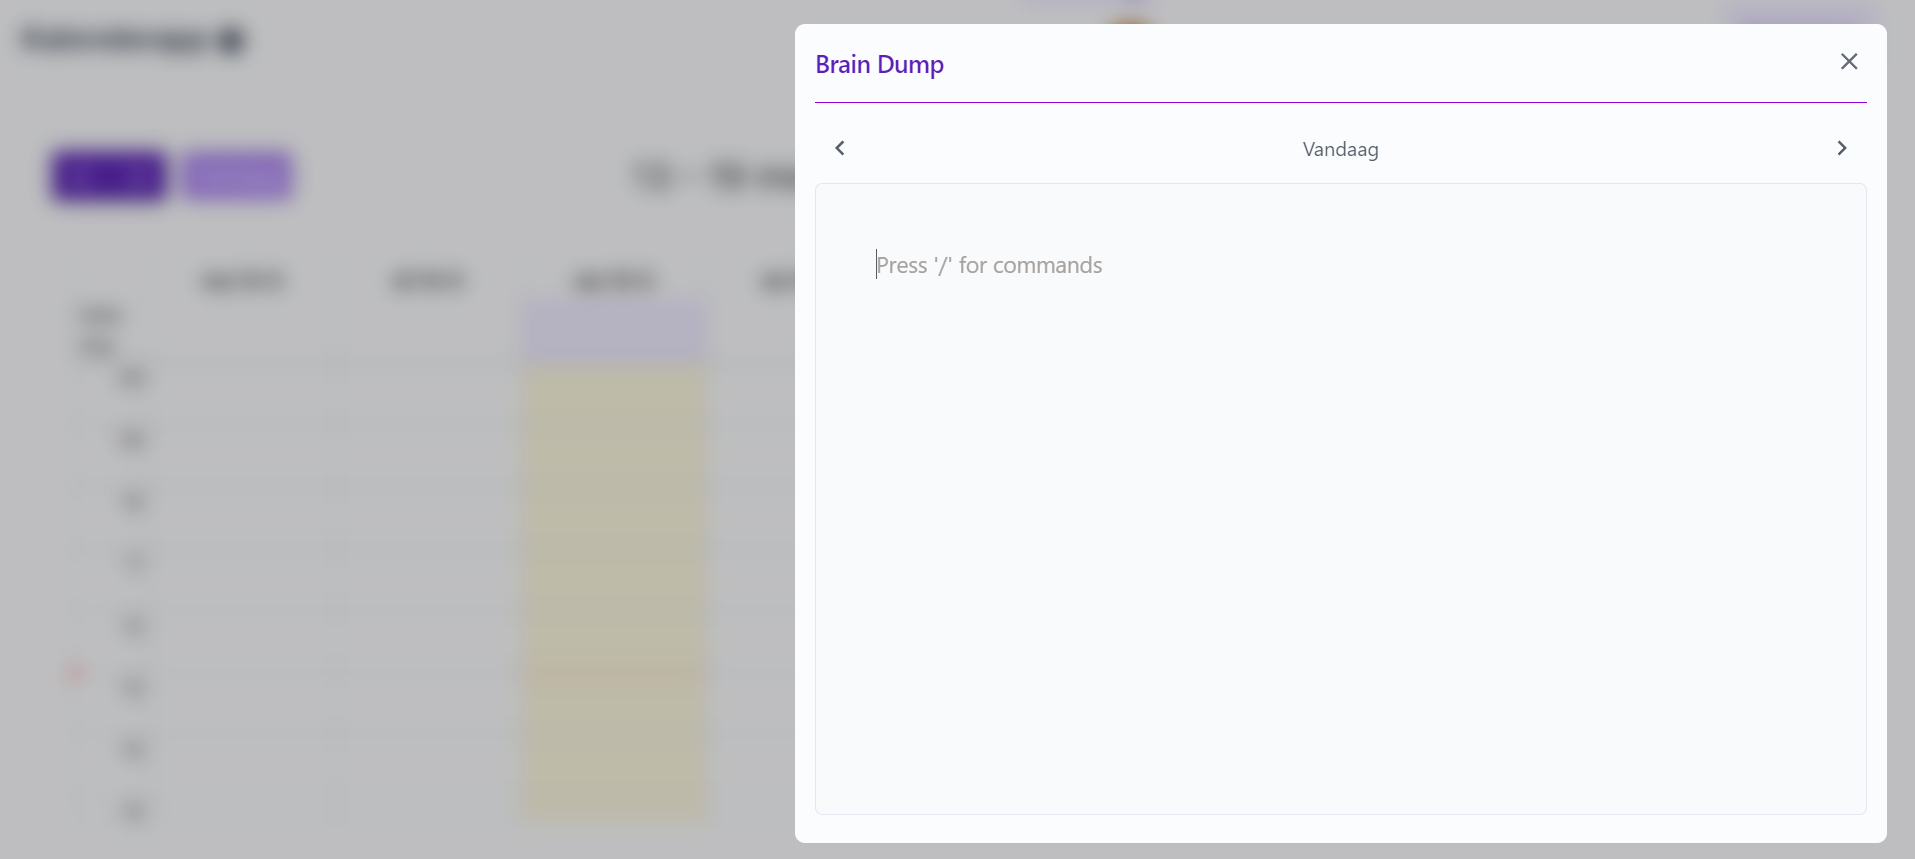
\includegraphics[width=\textwidth]{graphics/screenshot_braindump.png}
    \caption{Screenshot van de Brain Dump.}
    \label{fig:screenshot_braindump}
\end{figure}

\subsubsection{Overzicht in te plannen zaken}

Voor deze functionaliteit is geen nieuwe externe bibliotheek vereist; deze is volledig ontwikkeld met React-code en de 'Draggable'-eigenschap uit de FullCalendar-bibliotheek. Hoewel de code zelf niet wordt weergegeven in deze sectie, wordt een beschrijving gegeven van het uiteindelijke resultaat en hoe dit kan worden bereikt. \newline

Allereerst moet er naast de kalendercomponent een kader worden gecreëerd waarin de versleepbare evenementen geplaatst kunnen worden. Dit kan worden gerealiseerd met een `<div>`-element en passende opmaak. \newline

Dit kader wordt vervolgens gevuld door over een lijst van evenementen te mappen, waarbij voor elk element een blok wordt gegenereerd in de juiste kleur die overeenkomt met de categorie van het evenement. Deze blokken kunnen versleepbaar worden gemaakt door de klasse 'draggable-el' toe te wijzen aan het gegenereerde blok tijdens de iteratie over de lijst. \newline

Bij het laden van de pagina worden alle elementen met deze klasse omgezet in versleepbare objecten. Dit kan worden bereikt door gebruik te maken van de 'useEffect-hook' van React. Binnen deze hook worden de elementen gefilterd die behoren tot de gewenste klasse en worden ze omgezet naar versleepbare elementen met behulp van de 'new Draggable' methode uit de FullCalendar-bibliotheek. \newline

Het kader met overzicht van alle in te plannen zaken ziet er als volgt uit (figuur 4.5):

\begin{figure}[h]
    \centering
    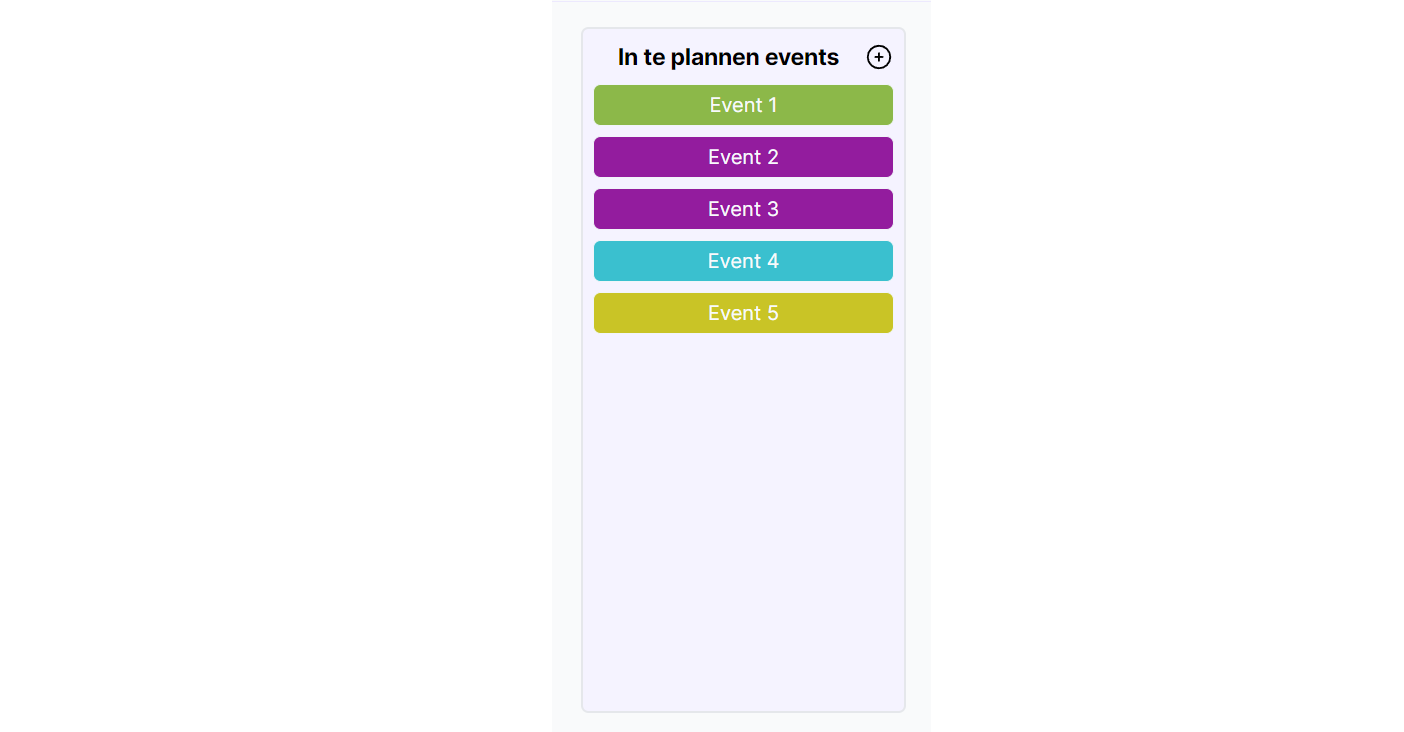
\includegraphics[width=\textwidth]{graphics/screenshot_overzicht.png}
    \caption{Screenshot van het Overzicht.}
    \label{fig:screenshot_overzicht}
\end{figure}


\subsubsection{Badges}

Als beloningssysteem in deze proof of concept zal een badgesysteem worden ontwikkeld. Dit systeem bestaat visueel uit een progressielijn tussen twee badges: de al verkregen badge van het vorige level en de te verkrijgen badge voor het volgende level. Daarboven zal er een knop aanwezig zijn die de verzameling behaalde badges toont, evenals een duidelijke weergave van het huidige level. \newline

Om dit op te zetten, is alleen het 'LinearProgress'-component van MUI nodig, terwijl de rest volledig kan worden ontworpen met React. \newline

De werking achter het badgesysteem in deze proof of concept is niet complex. Telkens wanneer een taak of evenement wordt voltooid, wordt deze toegevoegd aan een lijst. Op basis van deze lijst vordert de progressielijn. Zodra deze volledig is gevuld, gaat de gebruiker naar het volgende level en ontvangt deze een badge als beloning. Deze badge wordt ook toegevoegd aan de verzameling van de gebruiker, die te allen tijde kan worden geraadpleegd met behulp van de verzamelknop. \newline

Bij het halen van een nieuw level wordt de gebruiker ook gefeliciteerd en gemotiveerd om verder te doen. \newline

Hieronder vindt u de code voor het visualiseren van het badgesysteem, zonder styling.

\begin{lstlisting}[language=JavaScript, caption={Code Snippet - Badges}, label={lst:codesnippet4}, frame=single, breaklines=true, backgroundcolor=\color{lightgray}]
    <div>        
        <button onClick={() => setOpenCollection(true)}>
            Verzameling
        </button>
        <div>
            <Image alt="current" src={`/images/badgelvl${level}.png`}/>
            <LinearProgress variant="determinate" value={showProgressNumber} />    
            <Image alt="next" src={`/images/badgelvl${level + 1}.png`}/>
        </div>              
        <CongratulationDialog {...{ showCongratulations, setShowCongratulations, level }}/>
        <BadgeCollecion {...{ openCollection, setOpenCollection, level }}/>
    </div>
\end{lstlisting}

En hieronder krijgt u te zien hoe de progressielijn en motivatie eruitzien (figuur 4.6):

\begin{figure}[h]
    \centering
    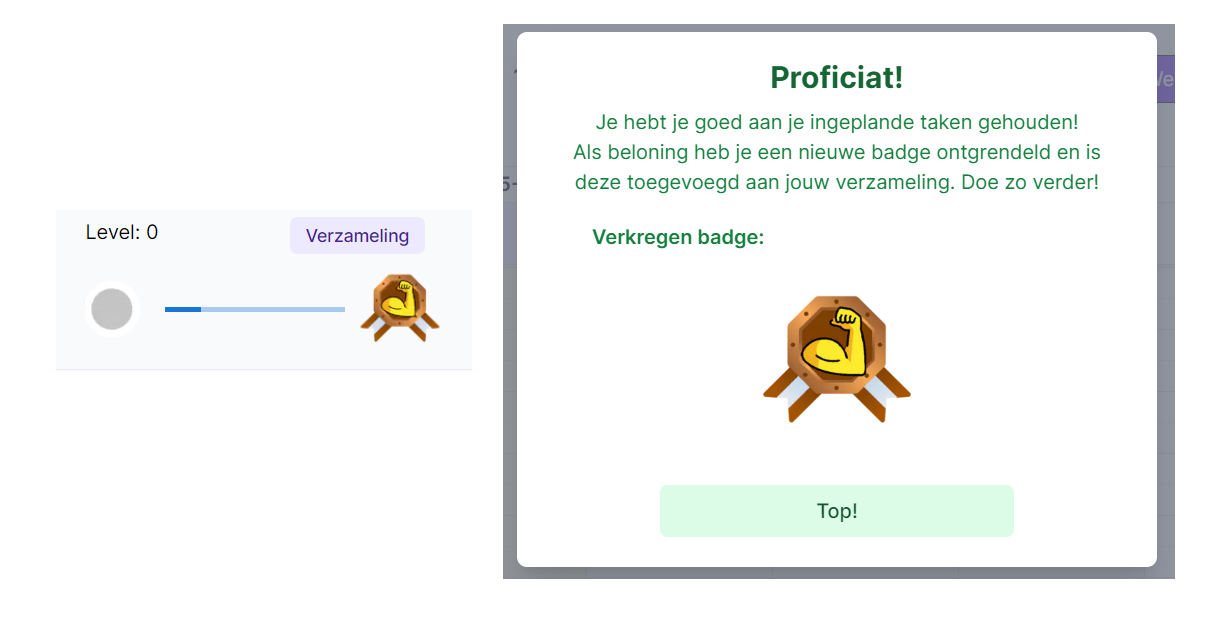
\includegraphics[width=\textwidth]{graphics/screenshot_badgesysteem.png}
    \caption{Screenshot van het Badgesysteem.}
    \label{fig:screenshot_badges}
\end{figure}


\subsubsection{Resultaat}
Als slot van deze sectie is er een screenshot van de gehele uitgewerkte applicatie (figuur 4.7). Nu dat deze volledig is uitgewerkt zal er in volgende sectie beschreven worden hoe deze applicatie getest zal worden in de praktijk. De resultaten van het onderzoek zullen later besproken en geïnterpreteerd worden.\newline
Figuur Proof of Concept: 

\begin{figure}[h]
    \centering
    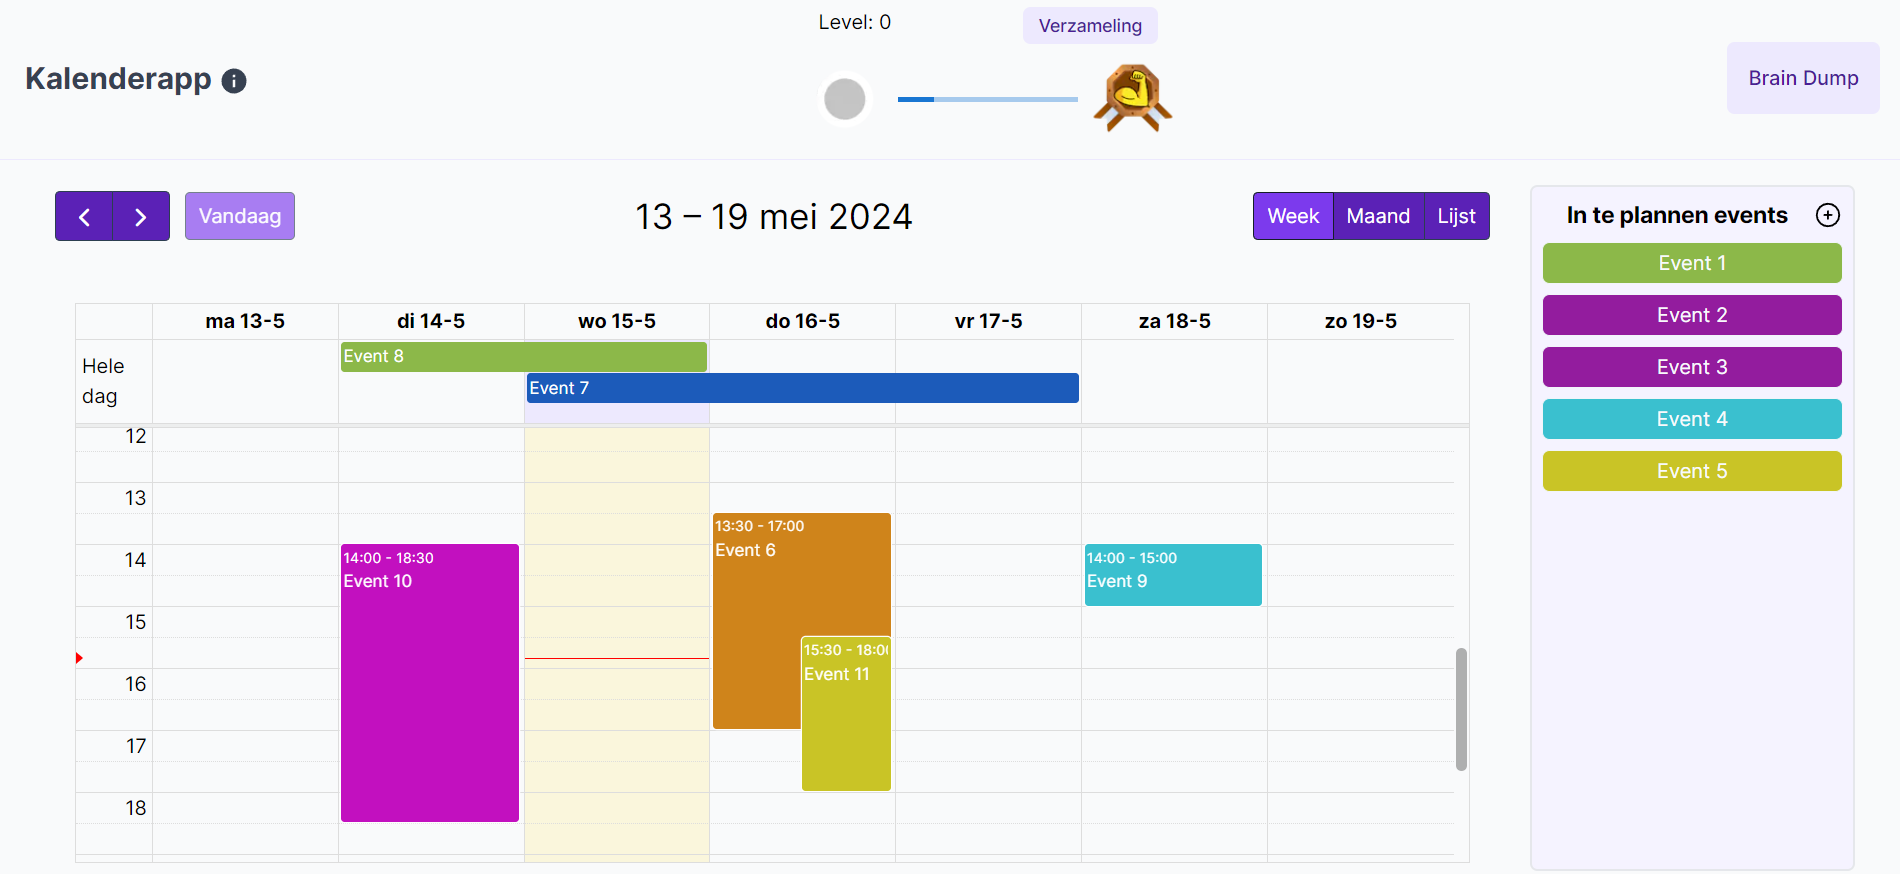
\includegraphics[width=\textwidth]{graphics/screenshot_applicatie.png}
    \caption{Screenshot van de Uitgewerkte Proof of Concept.}
    \label{fig:screenshot_applicatie}
\end{figure}

\subsection{Evaluatie van de applicatie}
Voor het testen van de proof of concept is er een evaluatieformulier opgesteld. Dit bevat bevragingen over de ontworpen features en de globale applicatie. Het formulier zal worden verspreid over de doelgroep die deze kritisch moet evalueren. In het formulier zit een link naar de applicatie die online draait en een handleiding om de applicatie volledig te kunnen testen. Er zal van de gebruikers verwacht worden om de aspecten en features een score te geven op 10. Er zal ook de mogelijkheid zijn om de kalenderapplicatie te vergelijken met een andere applicatie, die die de gebruiker op dit moment gebruikt bijvoorbeeld. Op basis van de scores en feedback zullen er conclusies worden getrokken. Dit is wat er in de volgende sectie zal gebeuren, het interpreteren van de resultaten.



\input{resultaten}

% Voeg hier je eigen hoofdstukken toe die de ``corpus'' van je bachelorproef
% vormen. De structuur en titels hangen af van je eigen onderzoek. Je kan bv.
% elke fase in je onderzoek in een apart hoofdstuk bespreken.

%\input{...}
%\input{...}
%...

%%=============================================================================
%% Conclusie
%%=============================================================================

\chapter{Conclusie}%
\label{ch:conclusie}

% TODO: Trek een duidelijke conclusie, in de vorm van een antwoord op de
% onderzoeksvra(a)g(en). Wat was jouw bijdrage aan het onderzoeksdomein en
% hoe biedt dit meerwaarde aan het vakgebied/doelgroep? 
% Reflecteer kritisch over het resultaat. In Engelse teksten wordt deze sectie
% ``Discussion'' genoemd. Had je deze uitkomst verwacht? Zijn er zaken die nog
% niet duidelijk zijn?
% Heeft het onderzoek geleid tot nieuwe vragen die uitnodigen tot verder 
%onderzoek?

\lipsum[76-80]



%---------- Bijlagen -----------------------------------------------------------

\appendix

\chapter{Onderzoeksvoorstel}

Het onderwerp van deze bachelorproef is gebaseerd op een onderzoeksvoorstel dat vooraf werd beoordeeld door de promotor. Dat voorstel is opgenomen in deze bijlage.

%% TODO: 
\section*{Samenvatting}
Dit onderzoek richt zich op het gebruik van inclusief ontwerp om een kalender applicatie te optimaliseren voor
mensen met AD(H)D. Deze soort applicaties zijn steeds meer noodzakelijk voor het verrichten en inplannen van
dagelijkse activiteiten door de hedendaagse drukte. Voor mensen met AD(H)D kan het gebruik van deze applicaties echter problematisch zijn vanwege hun complexiteit. Ze zijn vaak te overweldigend voor mensen met
AD(H)D omdat het ontwerp van de meeste applicaties niet gericht is op hun specifieke behoeften.
Het onderzoek begint met het identificeren van deze behoeften. Vervolgens worden er richtlijnen en beste praktijken opgesteld die aan deze behoeften voldoen voor het inclusief ontwerp. Eens deze richtlijnen zijn opgesteld
kan men de ontwerpen hier op afstemmen en zal er een applicatie ontwikkeld worden die later getest zal worden.
De resultaten van dit onderzoek zullen inzicht geven in de benodigdheden binnen de digitale wereld voor mensen met AD(H)D en zullen ontwerpers in staat stellen om een inclusief ontwerp te maken dat voor iedereen
toegankelijk is. Uit dit onderzoek zal men waarschijnlijk kunnen concluderen dat het gebruik van onder andere
eenvoudige en logische ordening, duidelijke sjablonen en visuele elementen dit doelpubliek al sterk kan helpen
bij het gebruik van deze applicaties.


% Kopieer en plak hier de samenvatting (abstract) van je onderzoeksvoorstel.

% Verwijzing naar het bestand met de inhoud van het onderzoeksvoorstel
%---------- Inleiding ---------------------------------------------------------

\section{Introductie}%
\label{sec:introductie}
In een wereld die steeds digitaler wordt zijn planning applicaties een handige tool voor het inplannen van dagelijkse activiteiten en het bijhouden van afspraken, deadlines etc. Deze applicaties zijn echter niet altijd even toegankelijk voor alle gebruikers, onder andere voor mensen met ADD. Deze groep individuen ervaart vaak moeilijkheden bij het gebruik van deze applicaties want vaak zijn ze te overweldigend en ingewikkeld. Dit komt omdat ze ontworpen zijn voor de gemiddelde mens. In dit onderzoek tracht ik deze moeilijkheden te verlichten volgens Inclusive Design. Omdat mensen met ADD nood hebben aan een goede planning om taken gedaan te krijgen, is dit onderzoek van belang. \newline \newline
Het ontwerpen van planning applicaties specifiek gericht op de behoeften en mogelijkheden van mensen met ADD is echter een complexe taak. Het vereist een diepgaand begrip van de individuele uitdagingen waarmee zij worden geconfronteerd. Het identificeren en verlichten van deze uitdagingen vereist samenwerking op het gebied van design, ontwikkeling, psychologie en technologie. \newline \newline
Het doel van dit onderzoeksvoorstel is om een diepgaand begrip te verkrijgen van de behoeften, uitdagingen en mogelijkheden voor mensen met ADD bij het gebruik van planning applicaties. Hiermee wordt het mogelijk om specifieke ontwerpkeuzes te evalueren en optimaliseren voor deze doelgroep. \newline \newline
Het uiteindelijke resultaat van dit onderzoeksvoorstel is het ontwikkelen van concrete aanbevelingen en richtlijnen voor het ontwerpen van planning applicaties die optimaal aansluiten bij de behoeften van mensen met ADD. Deze aanbevelingen kunnen worden gebruikt door ontwerpers, ontwikkelaars en beleidsmakers om inclusieve technologische oplossingen te creëren die de participatie en zelfstandigheid van deze doelgroep bevordert.
Door dit onderzoek hopen we bij te dragen aan een meer inclusieve samenleving waarin iedereen gelijke kansen krijgt om actief deel te nemen en te profiteren van de mogelijkheden die technologie biedt.


%---------- Stand van zaken ---------------------------------------------------

\section{literatuurstudie}%
\label{sec:literatuurstudie}

\subsection{Inclusief design} % \textbf{Inclusief design } \newline
Inclusief design dateert van voor softwareontwikkeling. Om te begrijpen hoe we het kunnen toepassen op software, kan het nuttig zijn om het bij fysieke producten te onderzoeken \autocite{Clarkson2003}. Hoewel deze ontwerpkeuzes vaak niet rechtstreeks toepasselijk zijn op het ontwerp van applicaties, kunnen de denkwijzen en methodologieën nuttig zijn voor het begrijpen van de benodigdheden bij mensen met beperkingen \newline

\subsection{Beperking} %\textbf{Beperkingen } \newline
Om te weten waarmee mensen met ADD het moeilijk hebben, moeten we eerst de beperking zelf en hun gedrag los van de online wereld  begrijpen \autocite{VanHerwegen2019} . Hierbij is het belangrijk om eerst te begrijpen wat Attention Deficit Disorder precies inhoudt, waarna we verder de uitdagingen en benodigdheden van personen met ADD kunnen onderzoeken \autocite{diamond2005attention}.
\newline

\subsection{Beperking en technologie} %\textbf{Beperkingen en technologie} \newline
Om een concreter beeld te krijgen van welke uitdagingen mensen met ADD aangaan bij het gebruik van planning-applicaties, kunnen we ook kijken naar hoe ze omgaan met browser- \autocite{Harrysson2004} en mobiele \autocite{Rapp2019} applicaties. \newline

\subsection{Inclusief design toepassen} %\textbf{Inclusief design toepassen } \newline
Na het onderzoeken van de uitdagingen en benodigdheden die veroorzaakt worden door een concentratiestoornis, kunnen de richtlijnen van inclusief design binnen ICT \autocite{Gulliksen2004, Nicolle2001, Roessvoll2013} toegepast worden om de ervaring gebruiksvriendelijker te maken voor mensen met specifieke deze stoornis.


% Voor literatuurverwijzingen zijn er twee belangrijke commando's:
% \autocite{KEY} => (Auteur, jaartal) Gebruik dit als de naam van de auteur
%   geen onderdeel is van de zin.
% \textcite{KEY} => Auteur (jaartal)  Gebruik dit als de auteursnaam wel een
%   functie heeft in de zin (bv. ``Uit onderzoek door Doll & Hill (1954) bleek
%   ...'')

%---------- Methodologie ------------------------------------------------------
\section{Methodologie}%
\label{sec:methodologie}

De aanpak van dit onderzoek is opgesplitst in vijf fasen, namelijk: de literatuurstudie, een doelgroepanalyse, een ontwerpoptimalisatie, het ontwerp implementeren en data verzamelen en tot slot het trekken van conclusies en het formuleren van aanbevelingen. Hieronder volgt een toelichting van de besproken fases. \newline 


De eerste fase van het onderzoek omvat een uitgebreide literatuurstudie om een stevig theoretisch kader te ontwikkelen. Deze studie richt zich op relevante literatuur over de behoeften, uitdagingen en mogelijkheden van mensen met ADD bij het gebruik van planning applicaties. Daarnaast worden bestaande ontwerpprincipes, richtlijnen en methoden voor het ontwerpen van inclusieve applicaties geïdentificeerd en geanalyseerd. \newline 

In de tweede fase van het onderzoek wordt een grondige analyse van de doelgroep uitgevoerd. Dit omvat het verzamelen van kwantitatieve en kwalitatieve gegevens om inzicht te krijgen in onder andere de specifieke behoeften, vaardigheden en beperkingen van mensen met ADD. Verschillende onderzoeksmethoden kunnen worden toegepast, zoals enquêtes, interviews, observaties en gebruikerstests, maar ook academische onderzoeken. Deze gegevens zullen als basis voor het ontwerpproces dienen. \newline 

Op basis van de inzichten uit de literatuurstudie en de doelgroepanalyse begint de derde fase, waarin ontwerpoptimalisatie plaatsvindt. In deze fase worden ontwerpprincipes en richtlijnen geformuleerd die specifiek zijn afgestemd op de behoeften van de doelgroep. Dit omvat het identificeren van gebruiksvriendelijke en toegankelijke interface-elementen, het vereenvoudigen van complexe taken en het bevorderen van betrokkenheid en motivatie bij het gebruik van planning applicaties. \newline 

Na het definiëren van de ontwerpoptimalisaties gaat het onderzoek over naar de implementatiefase. Hier worden de ontwerpconcepten en verbeteringen geïmplementeerd in concrete planning applicaties. Deze applicaties worden vervolgens getest en geëvalueerd met de doelgroep. De verzamelde gegevens omvatten zowel kwantitatieve als kwalitatieve metingen, zoals gebruikerstevredenheid, gebruiksgemak, efficiëntie en effectiviteit van de applicaties. \newline 

In de laatste fase worden de verzamelde gegevens geanalyseerd en geïnterpreteerd. Op basis van deze analyse worden conclusies getrokken met betrekking tot de effectiviteit en bruikbaarheid van de ontwikkelde planning applicaties voor mensen met ADD. Daarnaast worden aanbevelingen geformuleerd voor verdere optimalisatie en verbetering van deze applicaties, evenals voor toekomstig onderzoek op dit gebied.


%---------- Verwachte resultaten ----------------------------------------------
\section{Verwacht resultaat, Conclusie}%
\label{sec:verwachte_resultaten_conclusie}

De verwachte resultaten omvatten het volgende: een heldere en intuïtieve gebruiksflow, waarbij er gebruik wordt gemaakt van duidelijke en herkenbare icoontjes om de navigatie te vergemakkelijken. Om de visuele belasting te verminderen, streven we naar schermen die niet te druk zijn. \newline
Er zal waarschijnlijk een extra focus liggen op personalisatie, waarbij gebruikers de mogelijkheid hebben om functies aan of uit te schakelen op basis van hun voorkeuren. Bijvoorbeeld, het activeren van de 'Todo'-optie terwijl notitie herinneringen uitgeschakeld kunnen worden. \newline
Bovendien zal er moeten gezorgd worden voor duidelijk verdeelde tabs, elk met specifieke taken en functies om een overzichtelijke structuur te bieden. \newline
 
Door deze aanpassingen wordt er gestreefd naar een geoptimaliseerde en op maat gemaakte gebruikerservaring die specifiek inspeelt op de behoeften van mensen met ADD. Hierdoor zal het gebruik van planning-apps effectiever en aangenamer worden en wil ik bijdragen aan de ontwikkeling van deze applicaties die optimaal aansluiten bij hun behoeften.



%%---------- Andere bijlagen --------------------------------------------------
% TODO: Voeg hier eventuele andere bijlagen toe. Bv. als je deze BP voor de
% tweede keer indient, een overzicht van de verbeteringen t.o.v. het origineel.
%\input{...}

%%---------- Backmatter, referentielijst ---------------------------------------

\backmatter{}

\setlength\bibitemsep{2pt} %% Add Some space between the bibliograpy entries
\printbibliography[heading=bibintoc]

\end{document}
